
\begin{frame}
	\frametitle{Piecewise Linear Method}

		Assume that the state in the cell is piecewise linear with some slope $s$. This gives a second-order accurate method.
		\begin{align*}
			\text{For } && x_{i-\half} < x_i < x_{i+\half}: &
			\quad \rho(x, t=t_n) = \rho_i^n + s_i^n(x - x_i)\\[.5em]			
			\text{For }&& t_n < t < t_{n+1}: &\quad \rho(x, t) = \rho_i^n +s_i^n(x -[x_i + u (t - t_n)])
		\end{align*}
%		
		The flux over the interface is then
%
		\begin{align*}
			f_{i-\half}(t) 	&= u \rho(x = x_{i-\half}, t)\\
						&= u \rho_{i-1} +  u s_i^n(\nicefrac{\Delta x}{2} - u(t-t_n))
		\end{align*}
%
		Finally averaging the fluxes over a time step gives:
		\begin{align*}
			\rho_i^{n+1} = \rho_i^n - \frac{u \Delta t}{\Delta x} ( \rho_i ^n - \rho_{i-1}^n) - \frac{u \Delta t}{\Delta x} \frac{1}{2} (s_i^n - s_{i-1}^n)(\Delta x - u\Delta t)
		\end{align*}
		
		Choice of slope: $s_i^n = \frac{\rho_{i+1}^n - \rho_i^n}{\Delta x}$ ( Lax-Wendroff method )

\end{frame}









\begin{frame}
	\vspace{10pt}
	\begin{columns}
		\column{.33\textwidth}
			\centering
			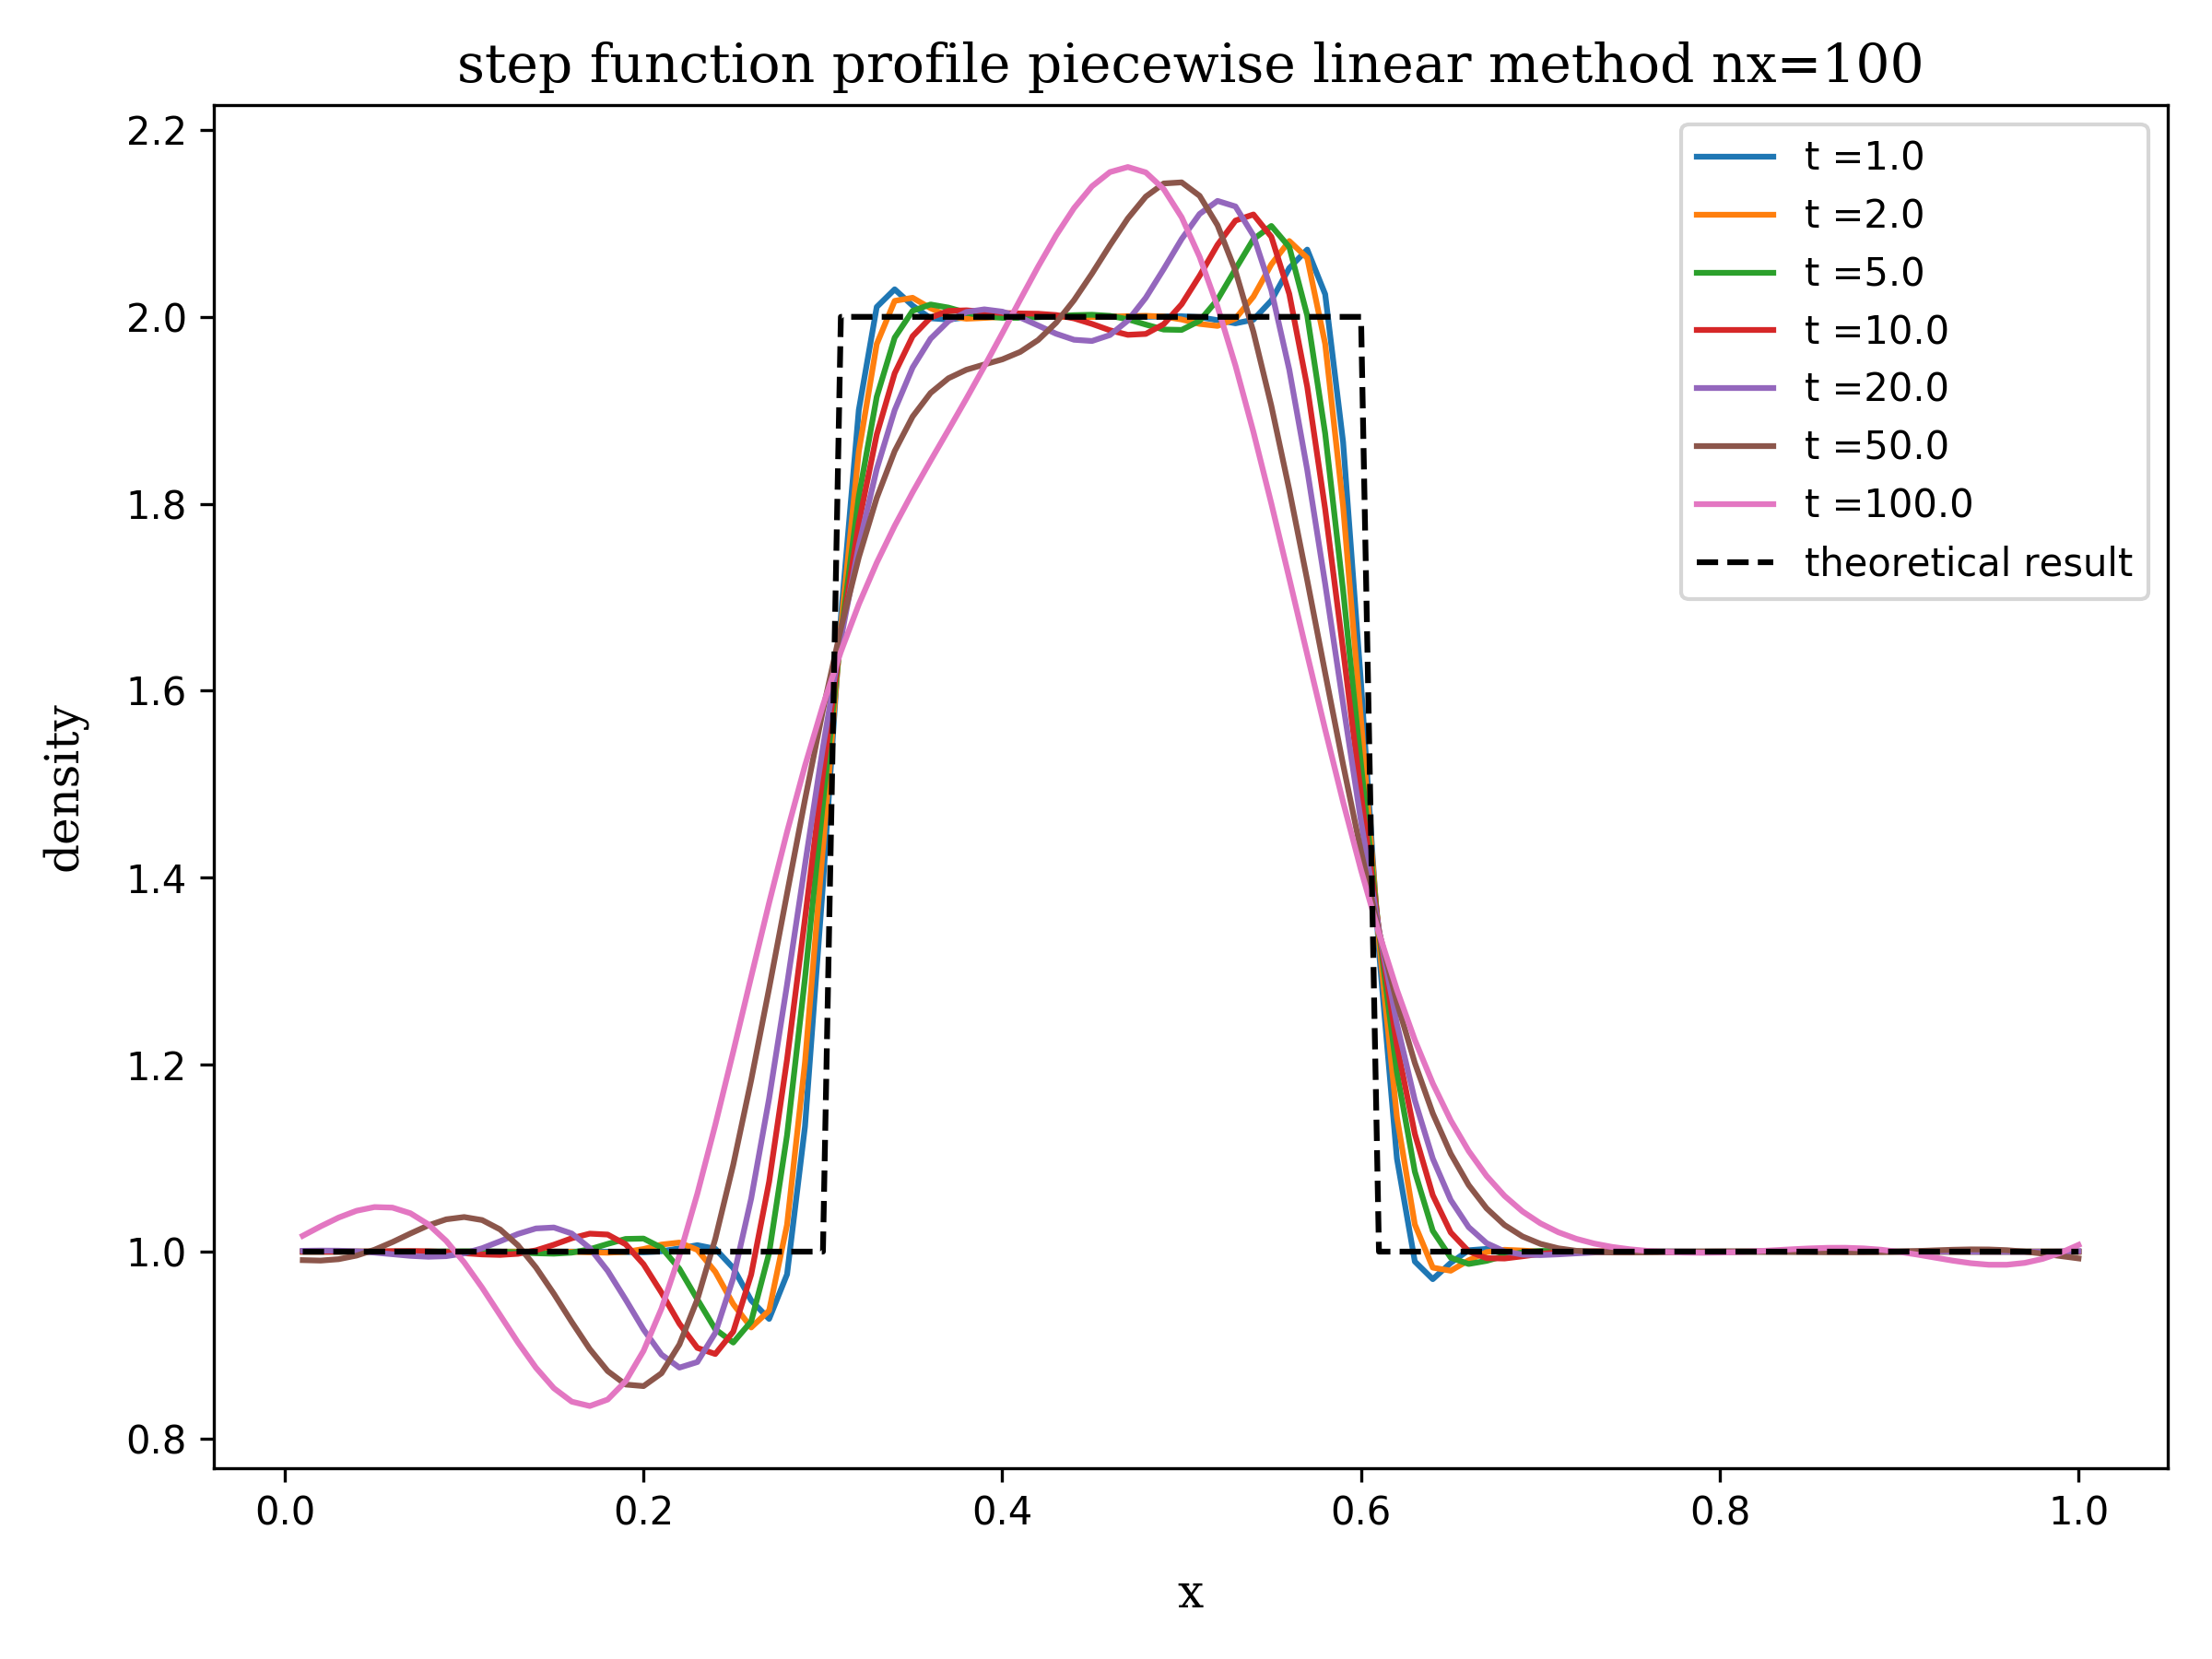
\includegraphics[height=.33\textheight]{../results/1D/pwlin/nx=100/plot_advection_step_function_pwlin_nx=100.png}\\
			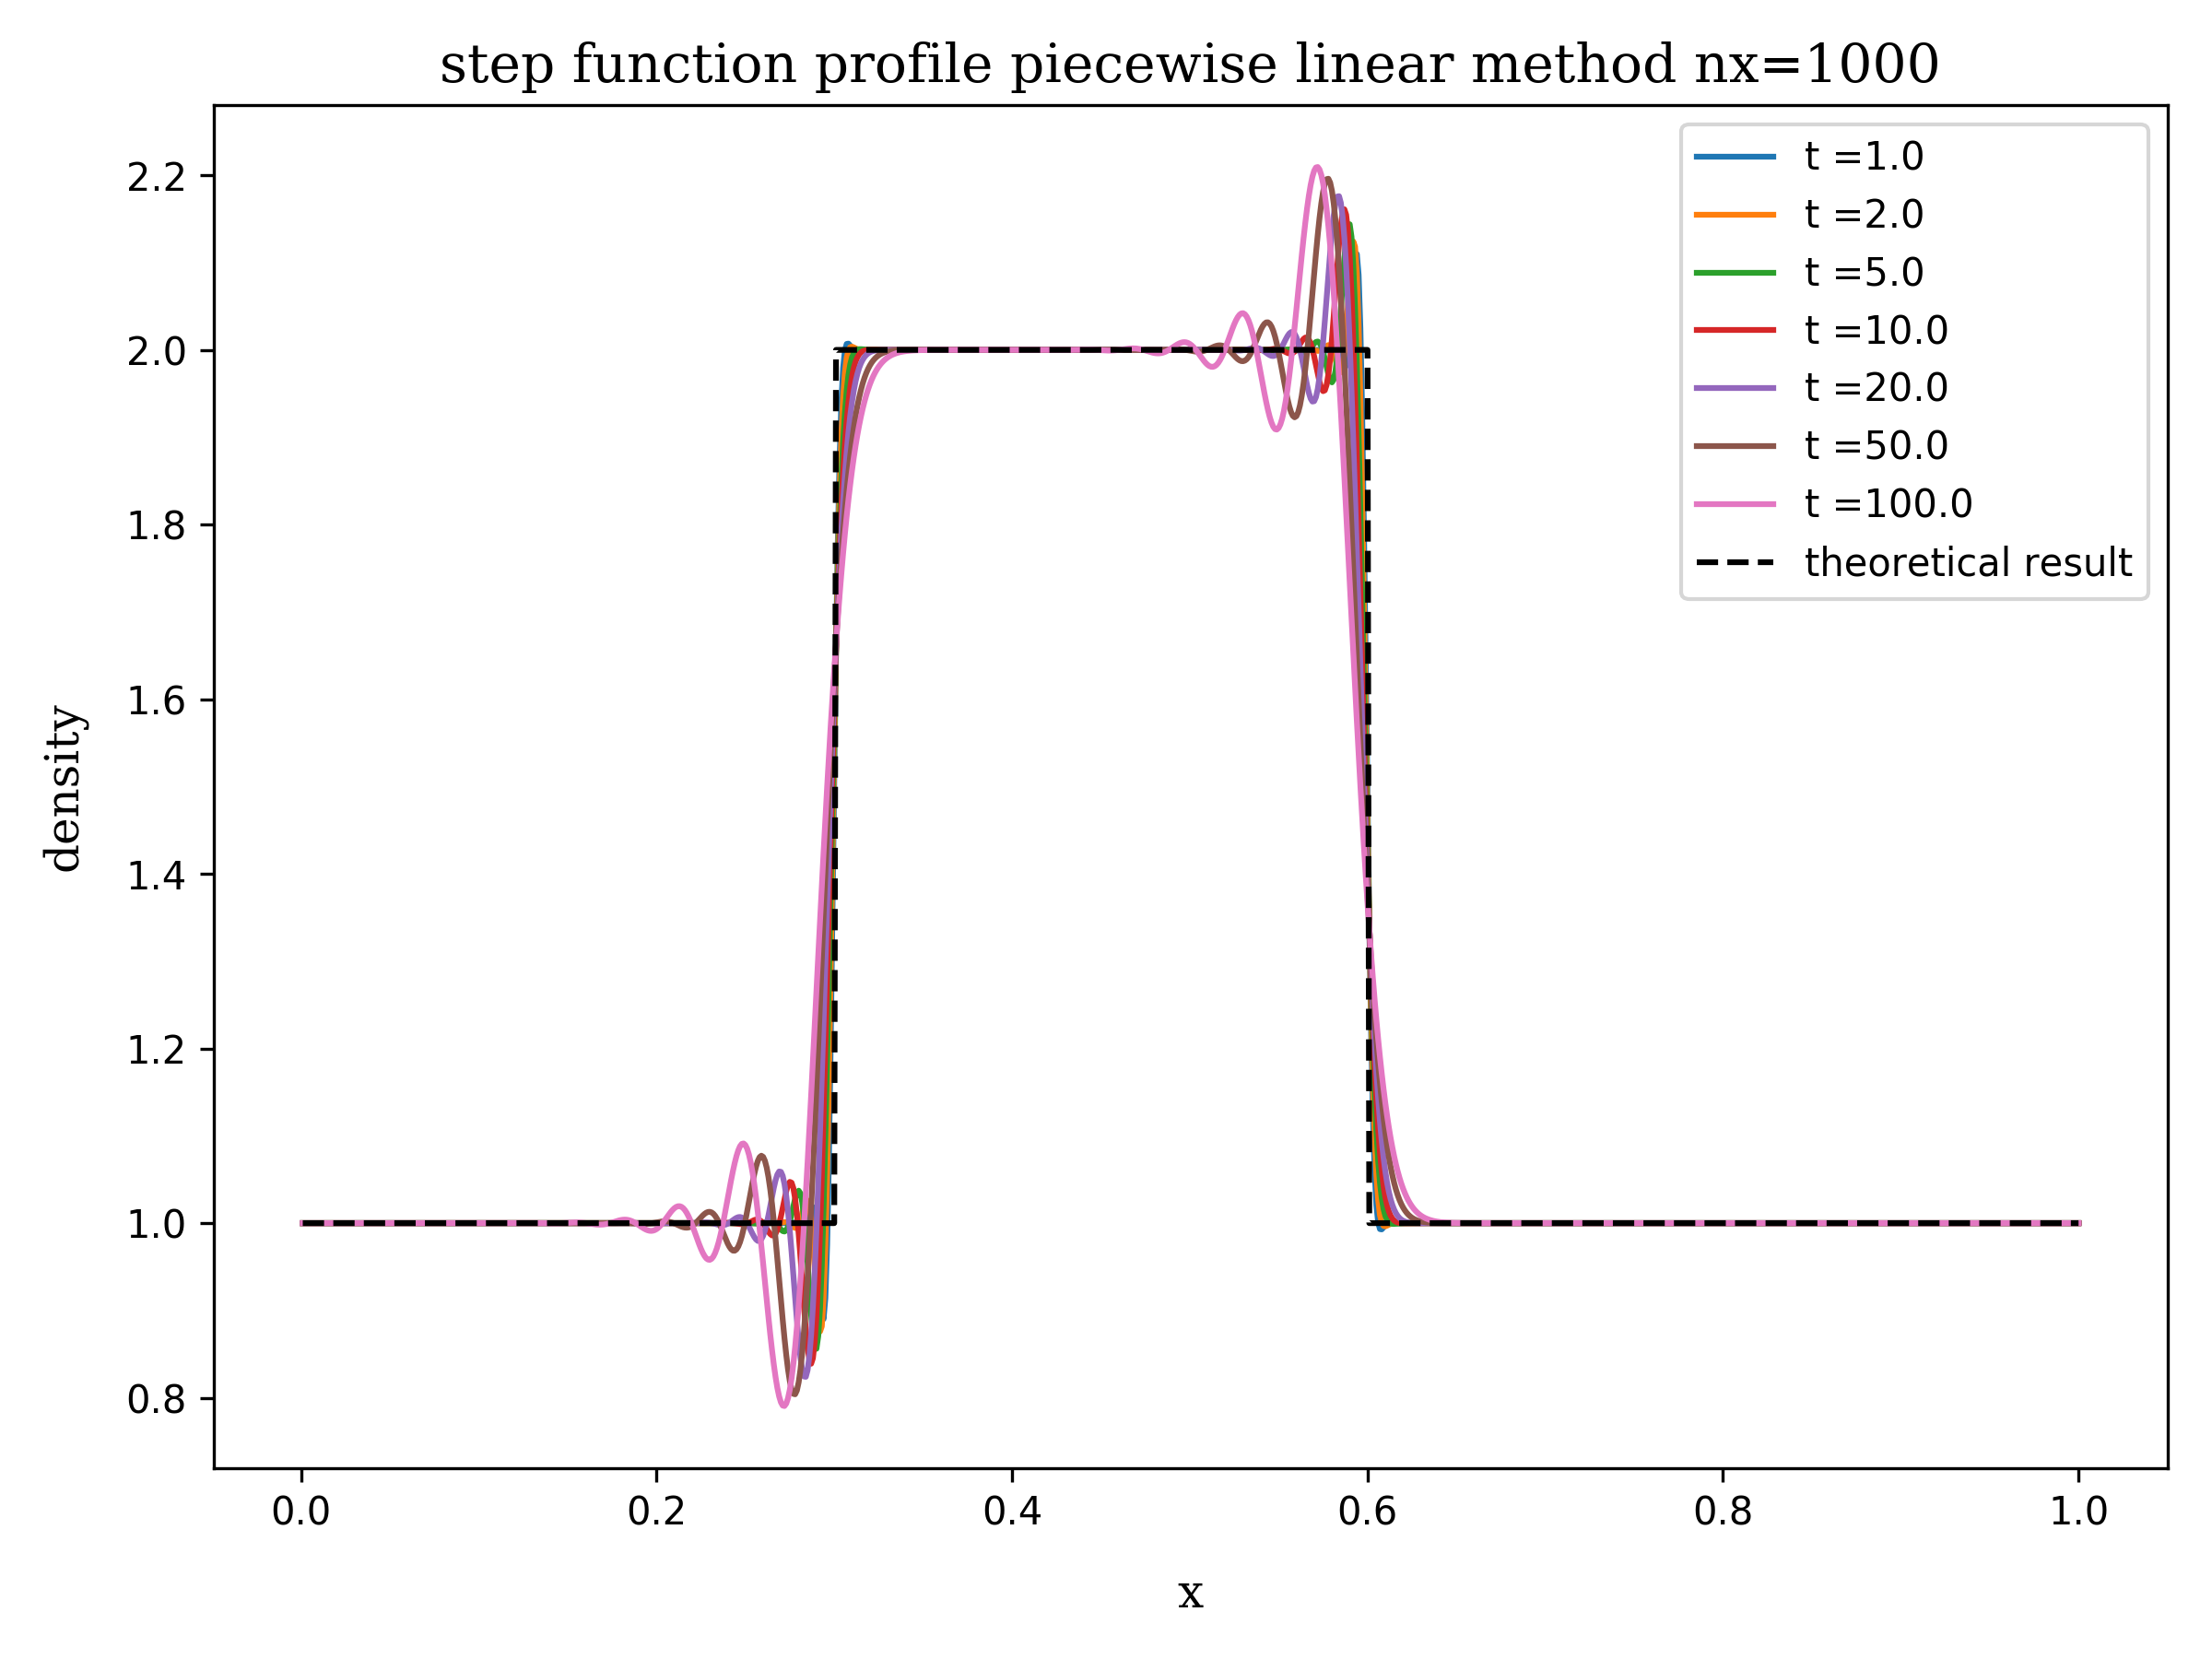
\includegraphics[height=.33\textheight]{../results/1D/pwlin/nx=1000/plot_advection_step_function_pwlin_nx=1000.png}\\
			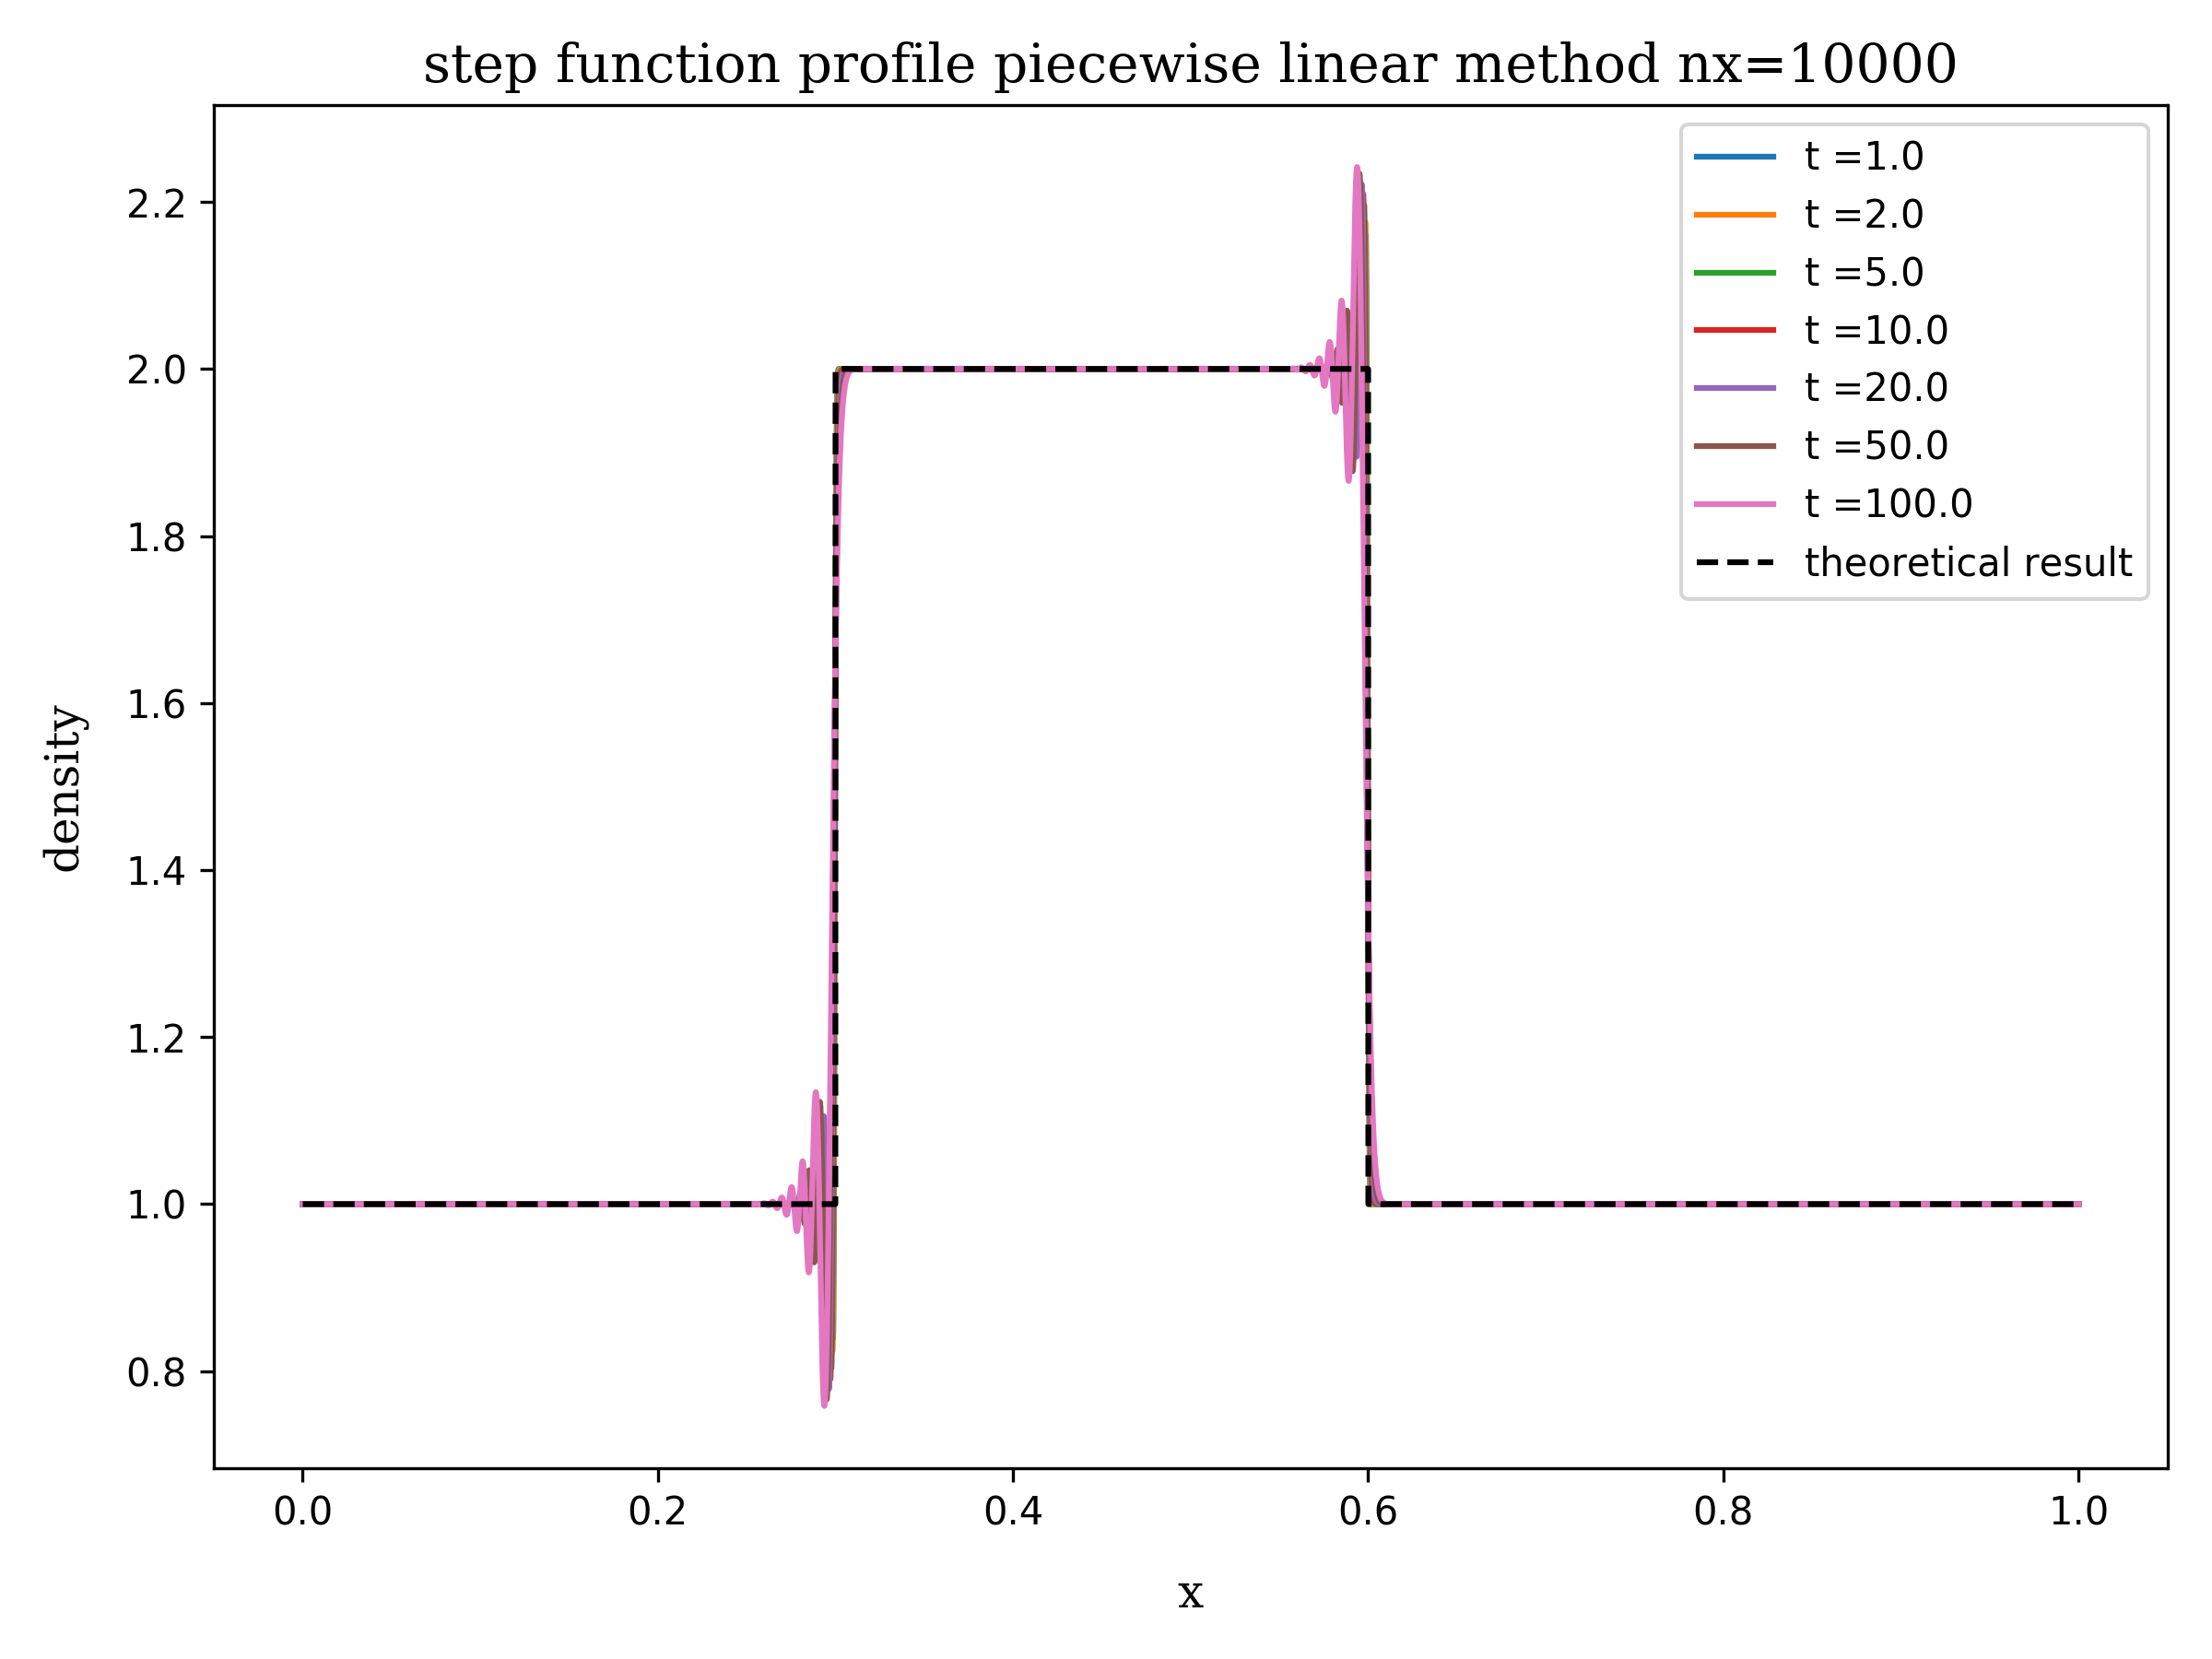
\includegraphics[height=.33\textheight]{../results/1D/pwlin/nx=10000/plot_advection_step_function_pwlin_nx=10000.png}
		\column{.33\textwidth}
			\centering
			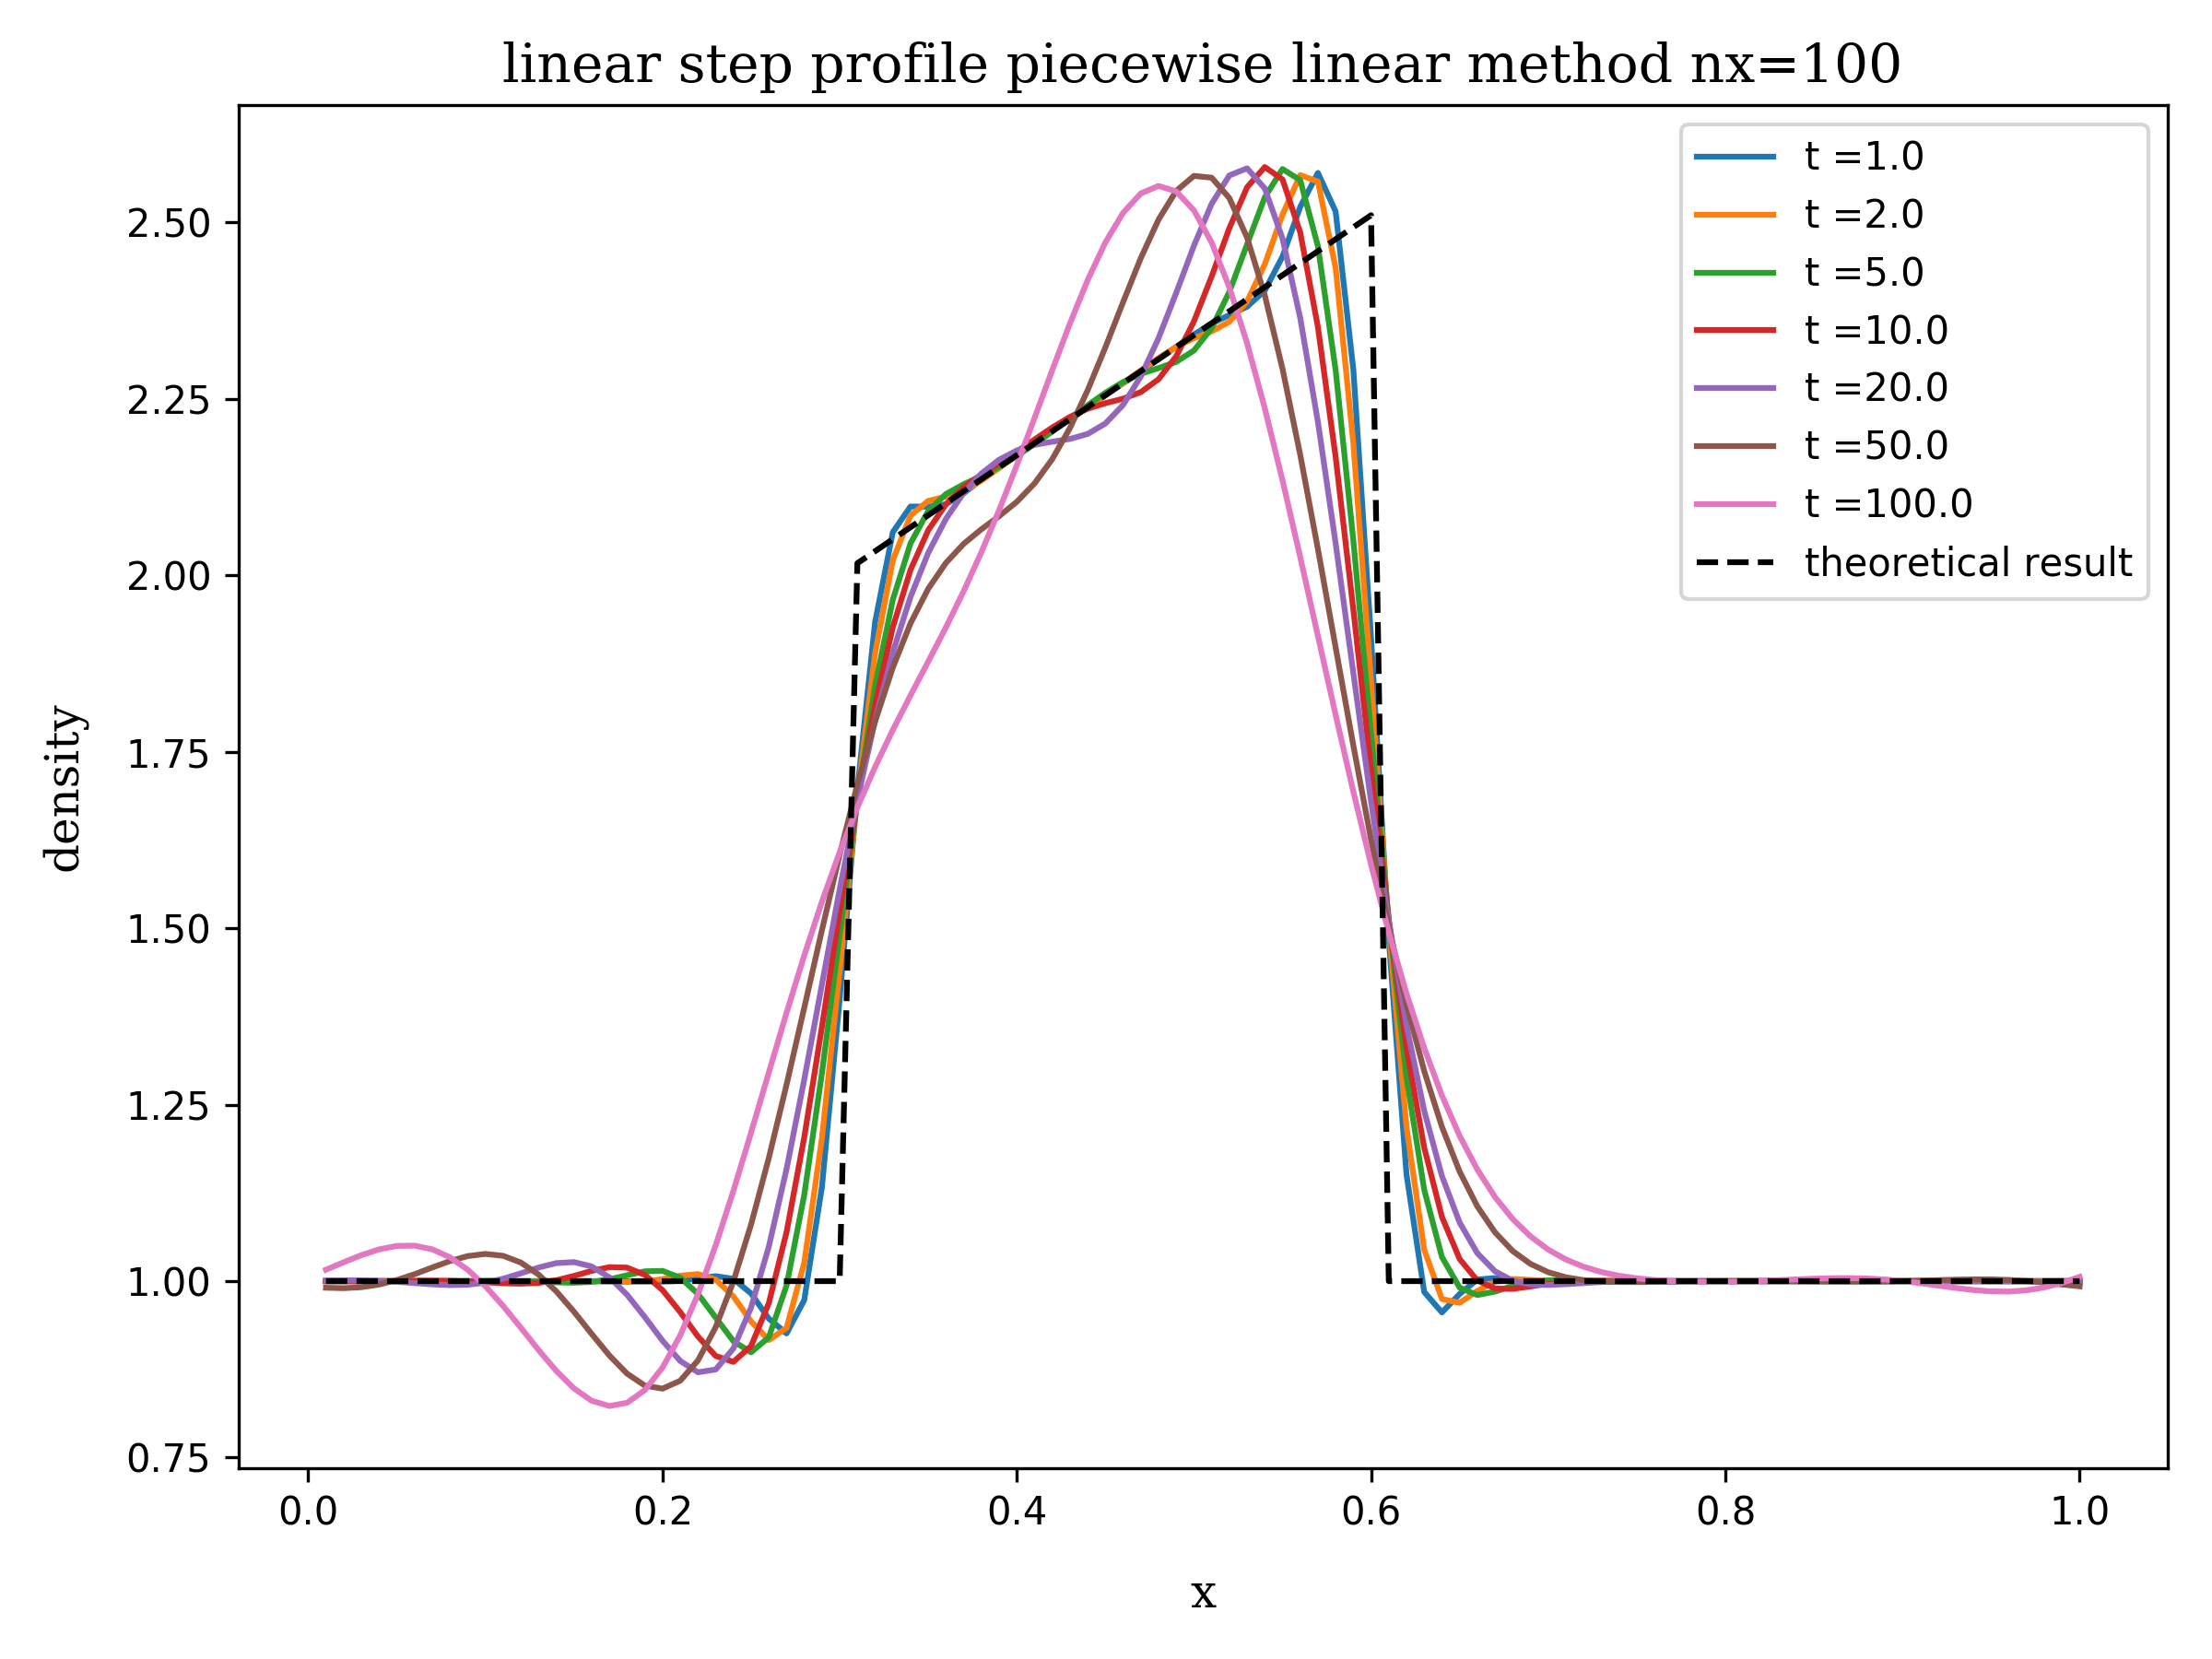
\includegraphics[height=.33\textheight]{../results/1D/pwlin/nx=100/plot_advection_linear_step_pwlin_nx=100.png}\\
			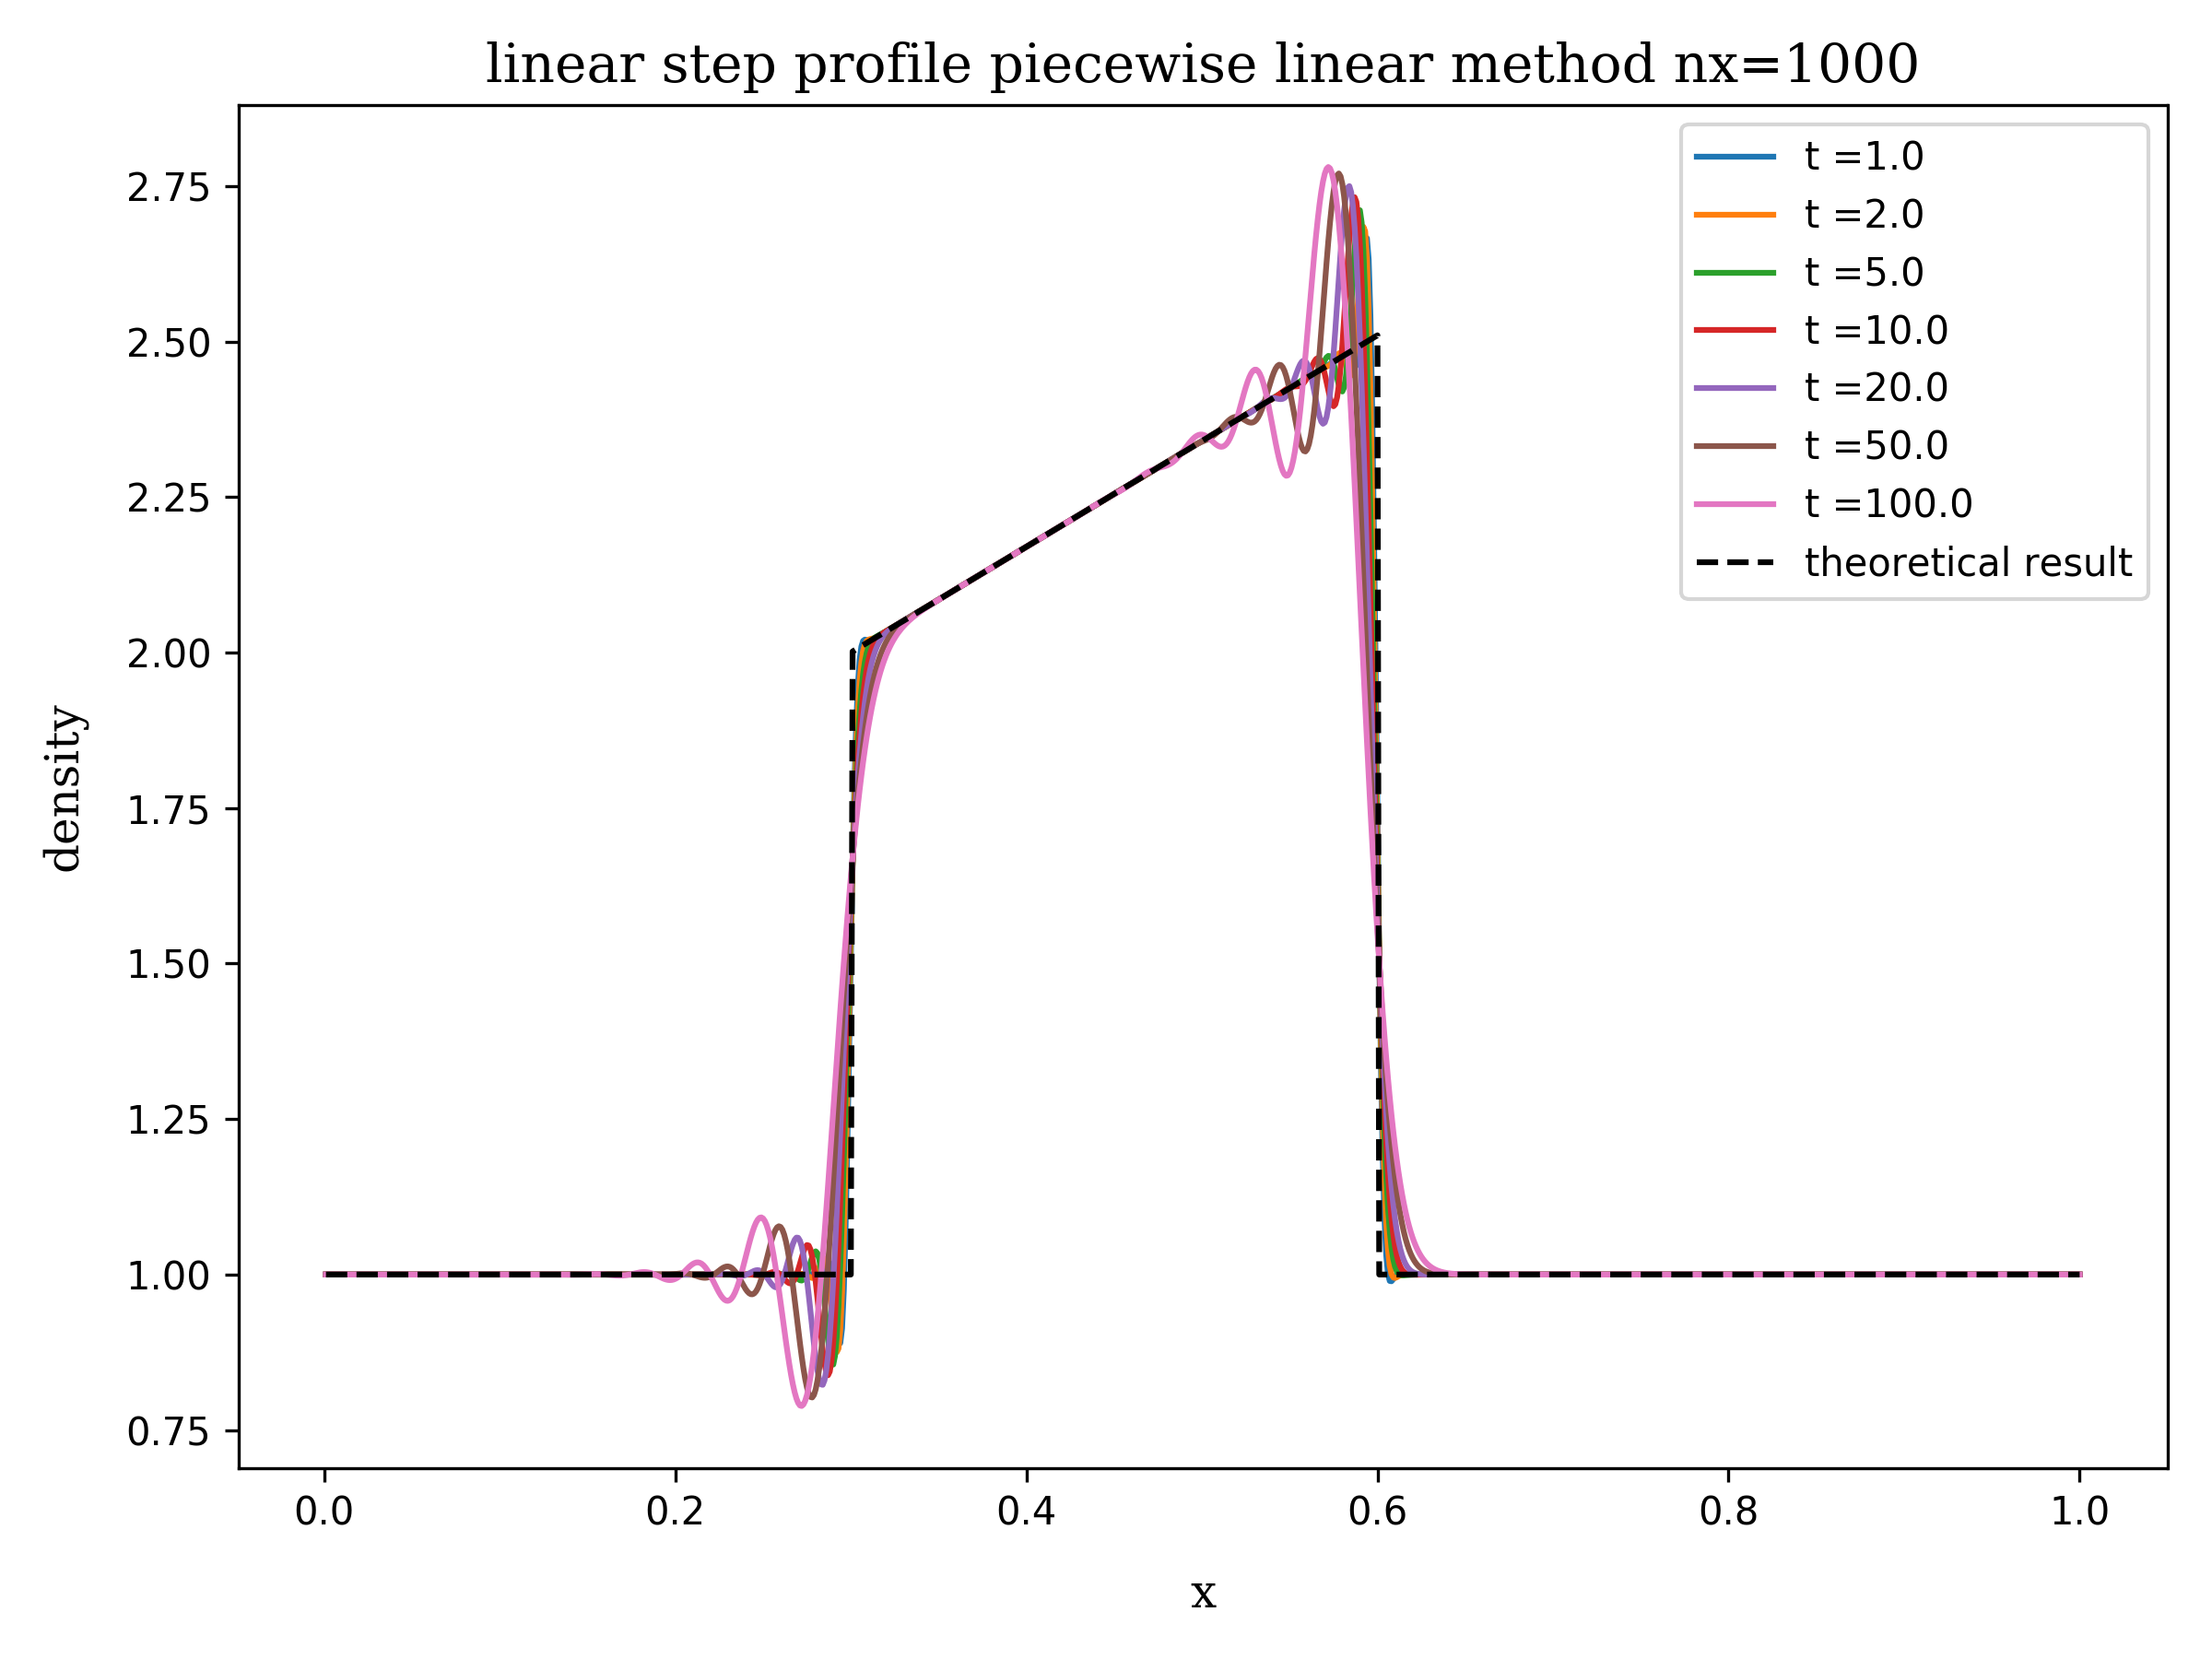
\includegraphics[height=.33\textheight]{../results/1D/pwlin/nx=1000/plot_advection_linear_step_pwlin_nx=1000.png}\\
			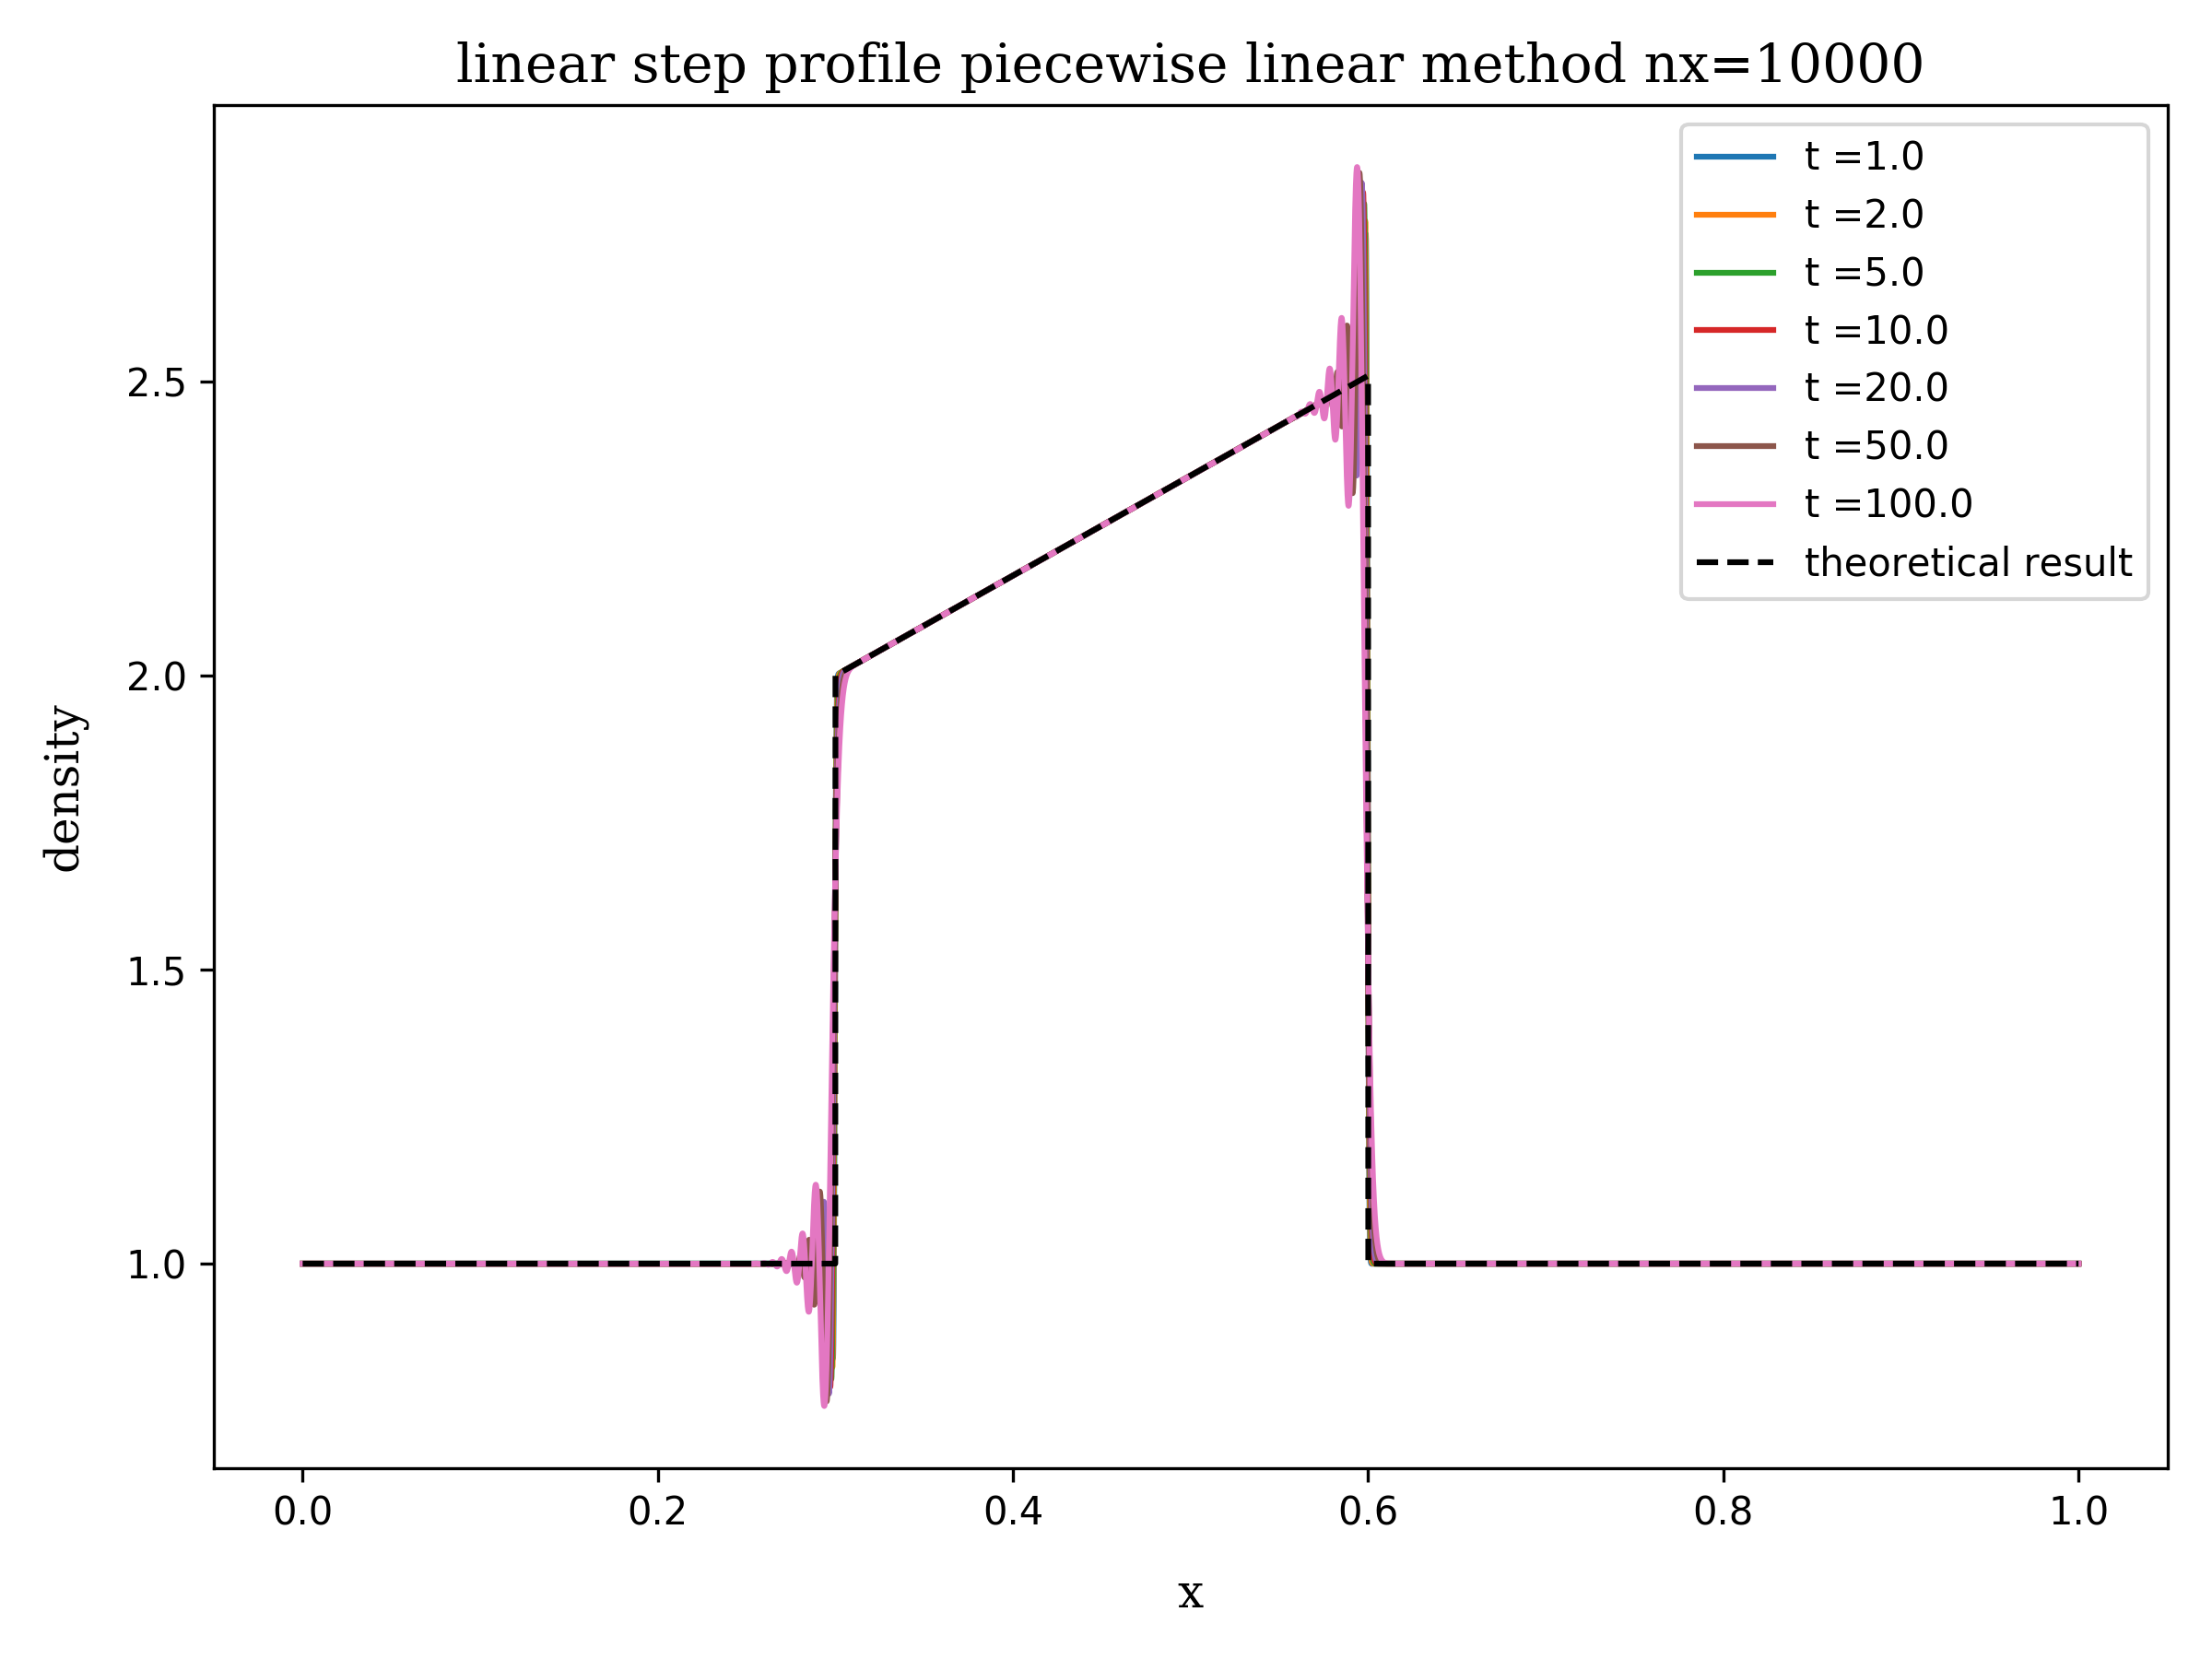
\includegraphics[height=.33\textheight]{../results/1D/pwlin/nx=10000/plot_advection_linear_step_pwlin_nx=10000.png}
		\column{.33\textwidth}
			\centering
			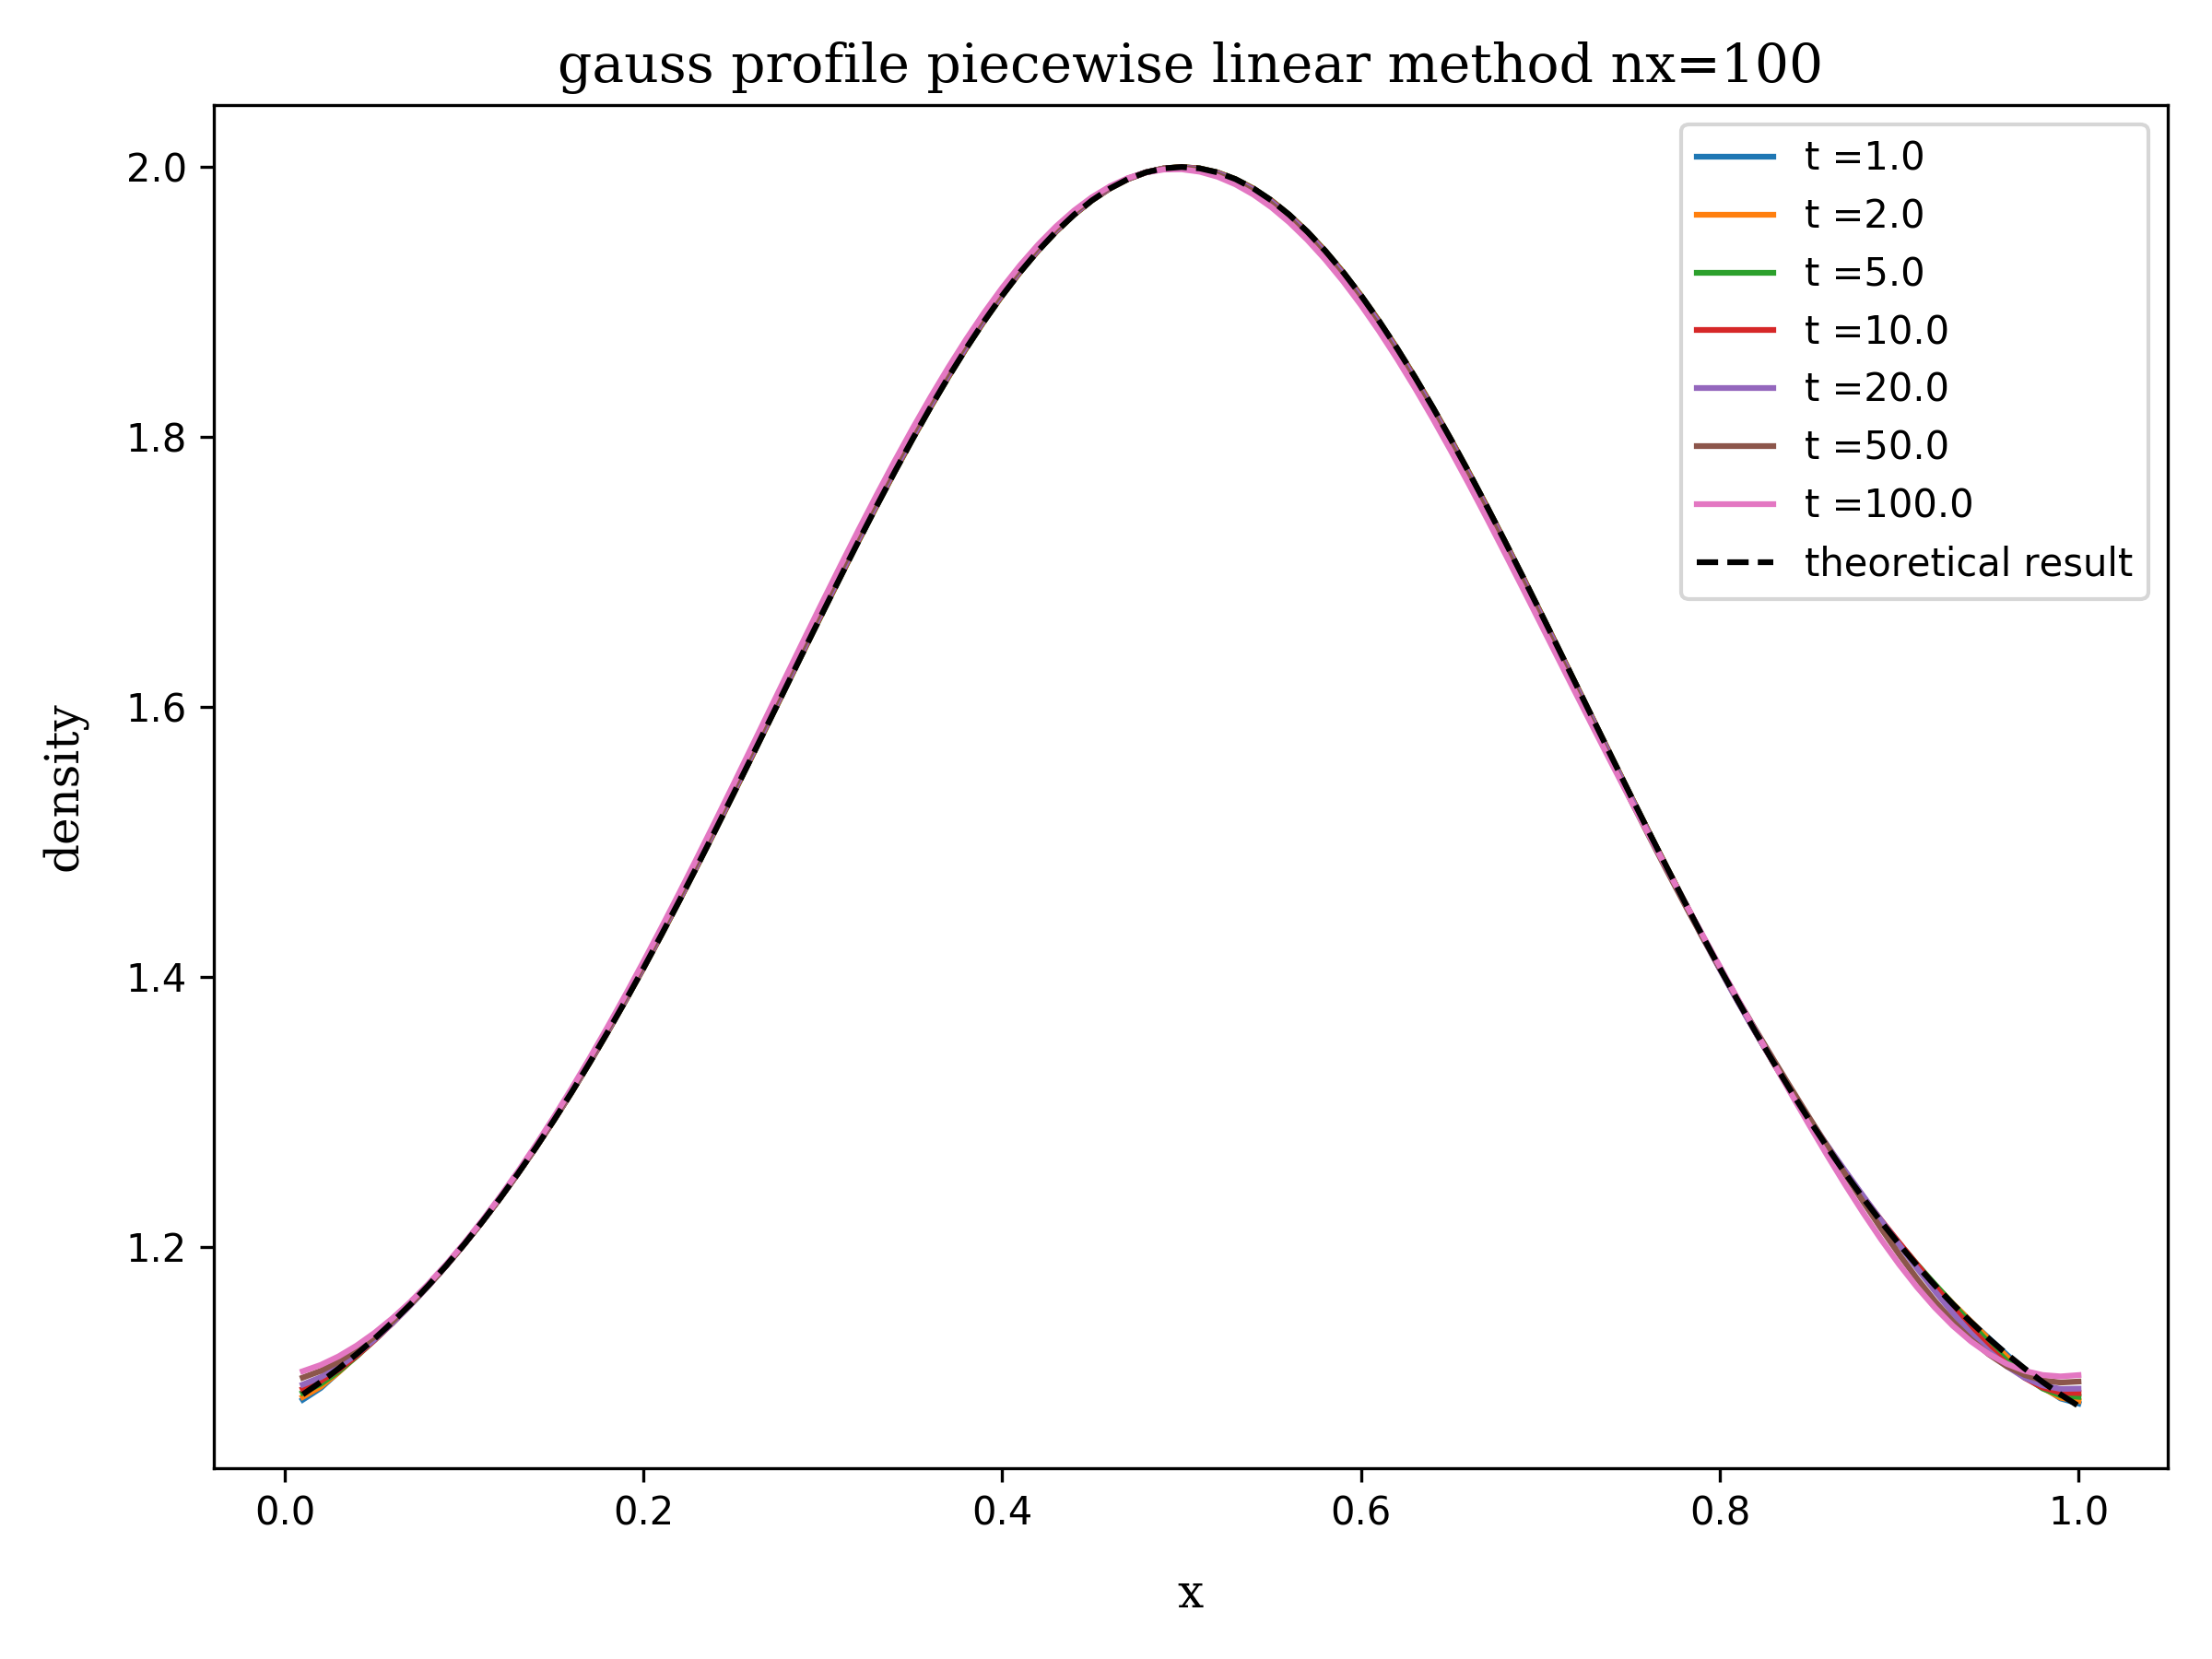
\includegraphics[height=.33\textheight]{../results/1D/pwlin/nx=100/plot_advection_gauss_pwlin_nx=100.png}\\
			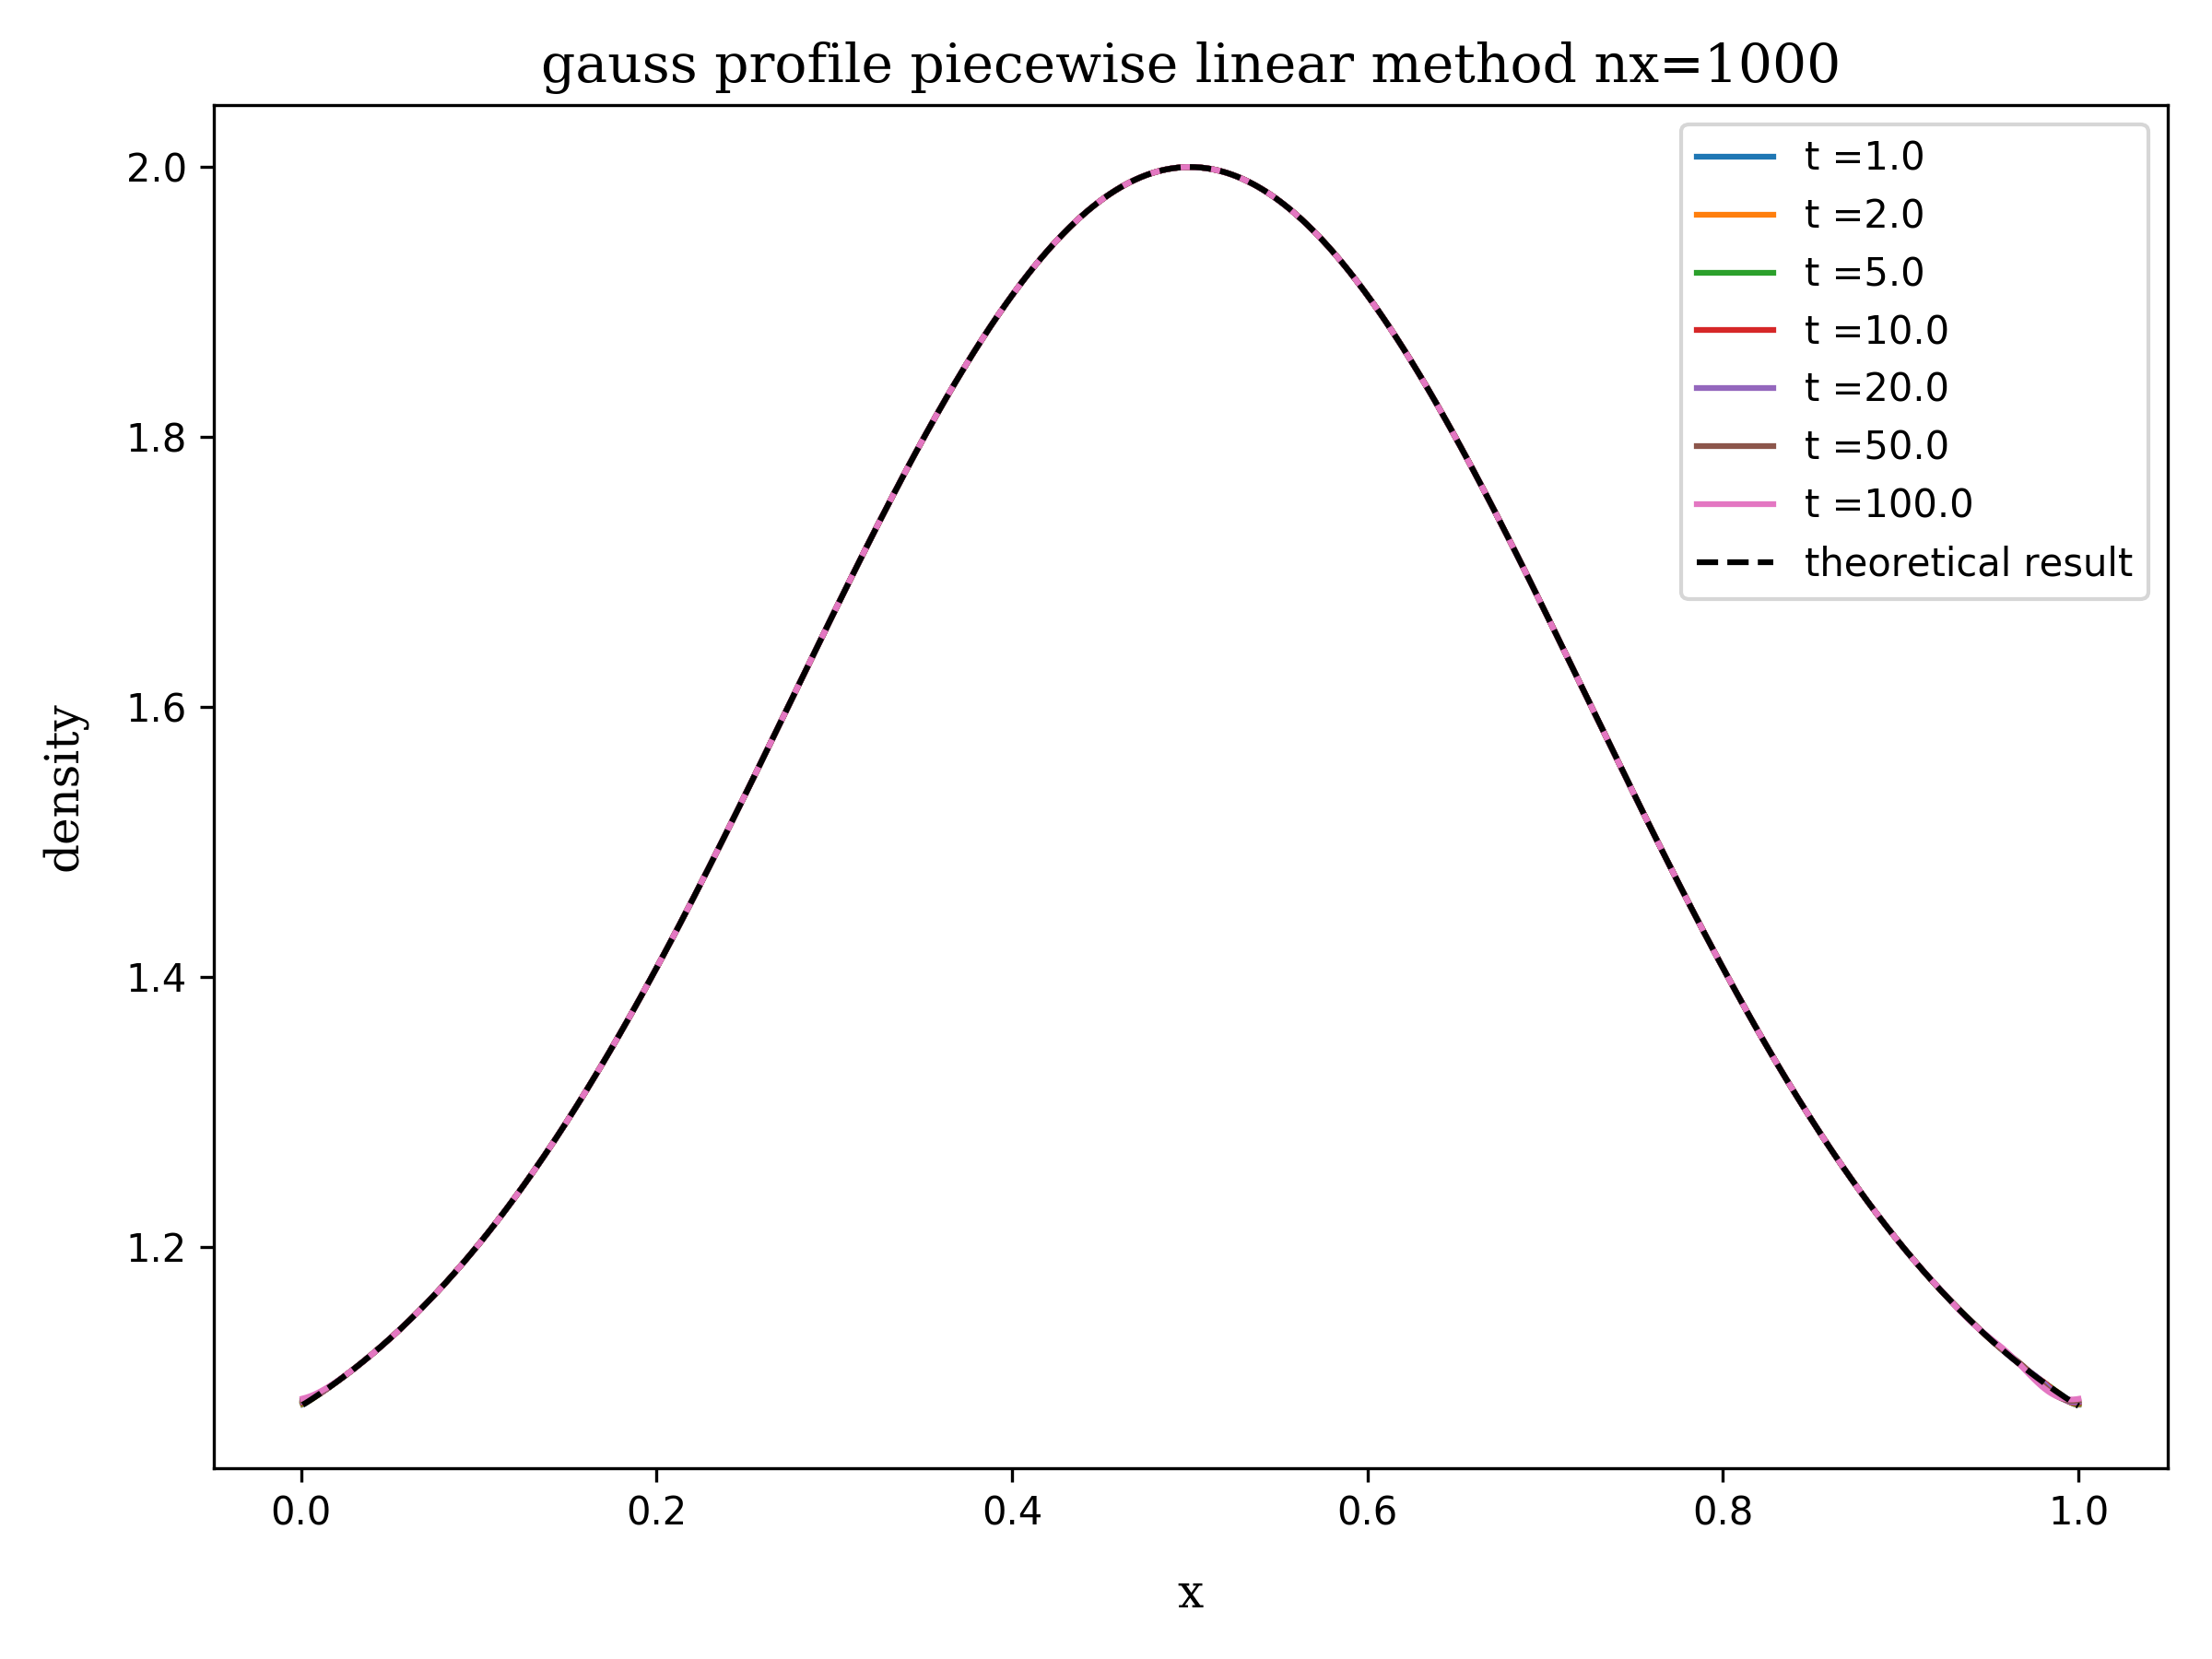
\includegraphics[height=.33\textheight]{../results/1D/pwlin/nx=1000/plot_advection_gauss_pwlin_nx=1000.png}\\
			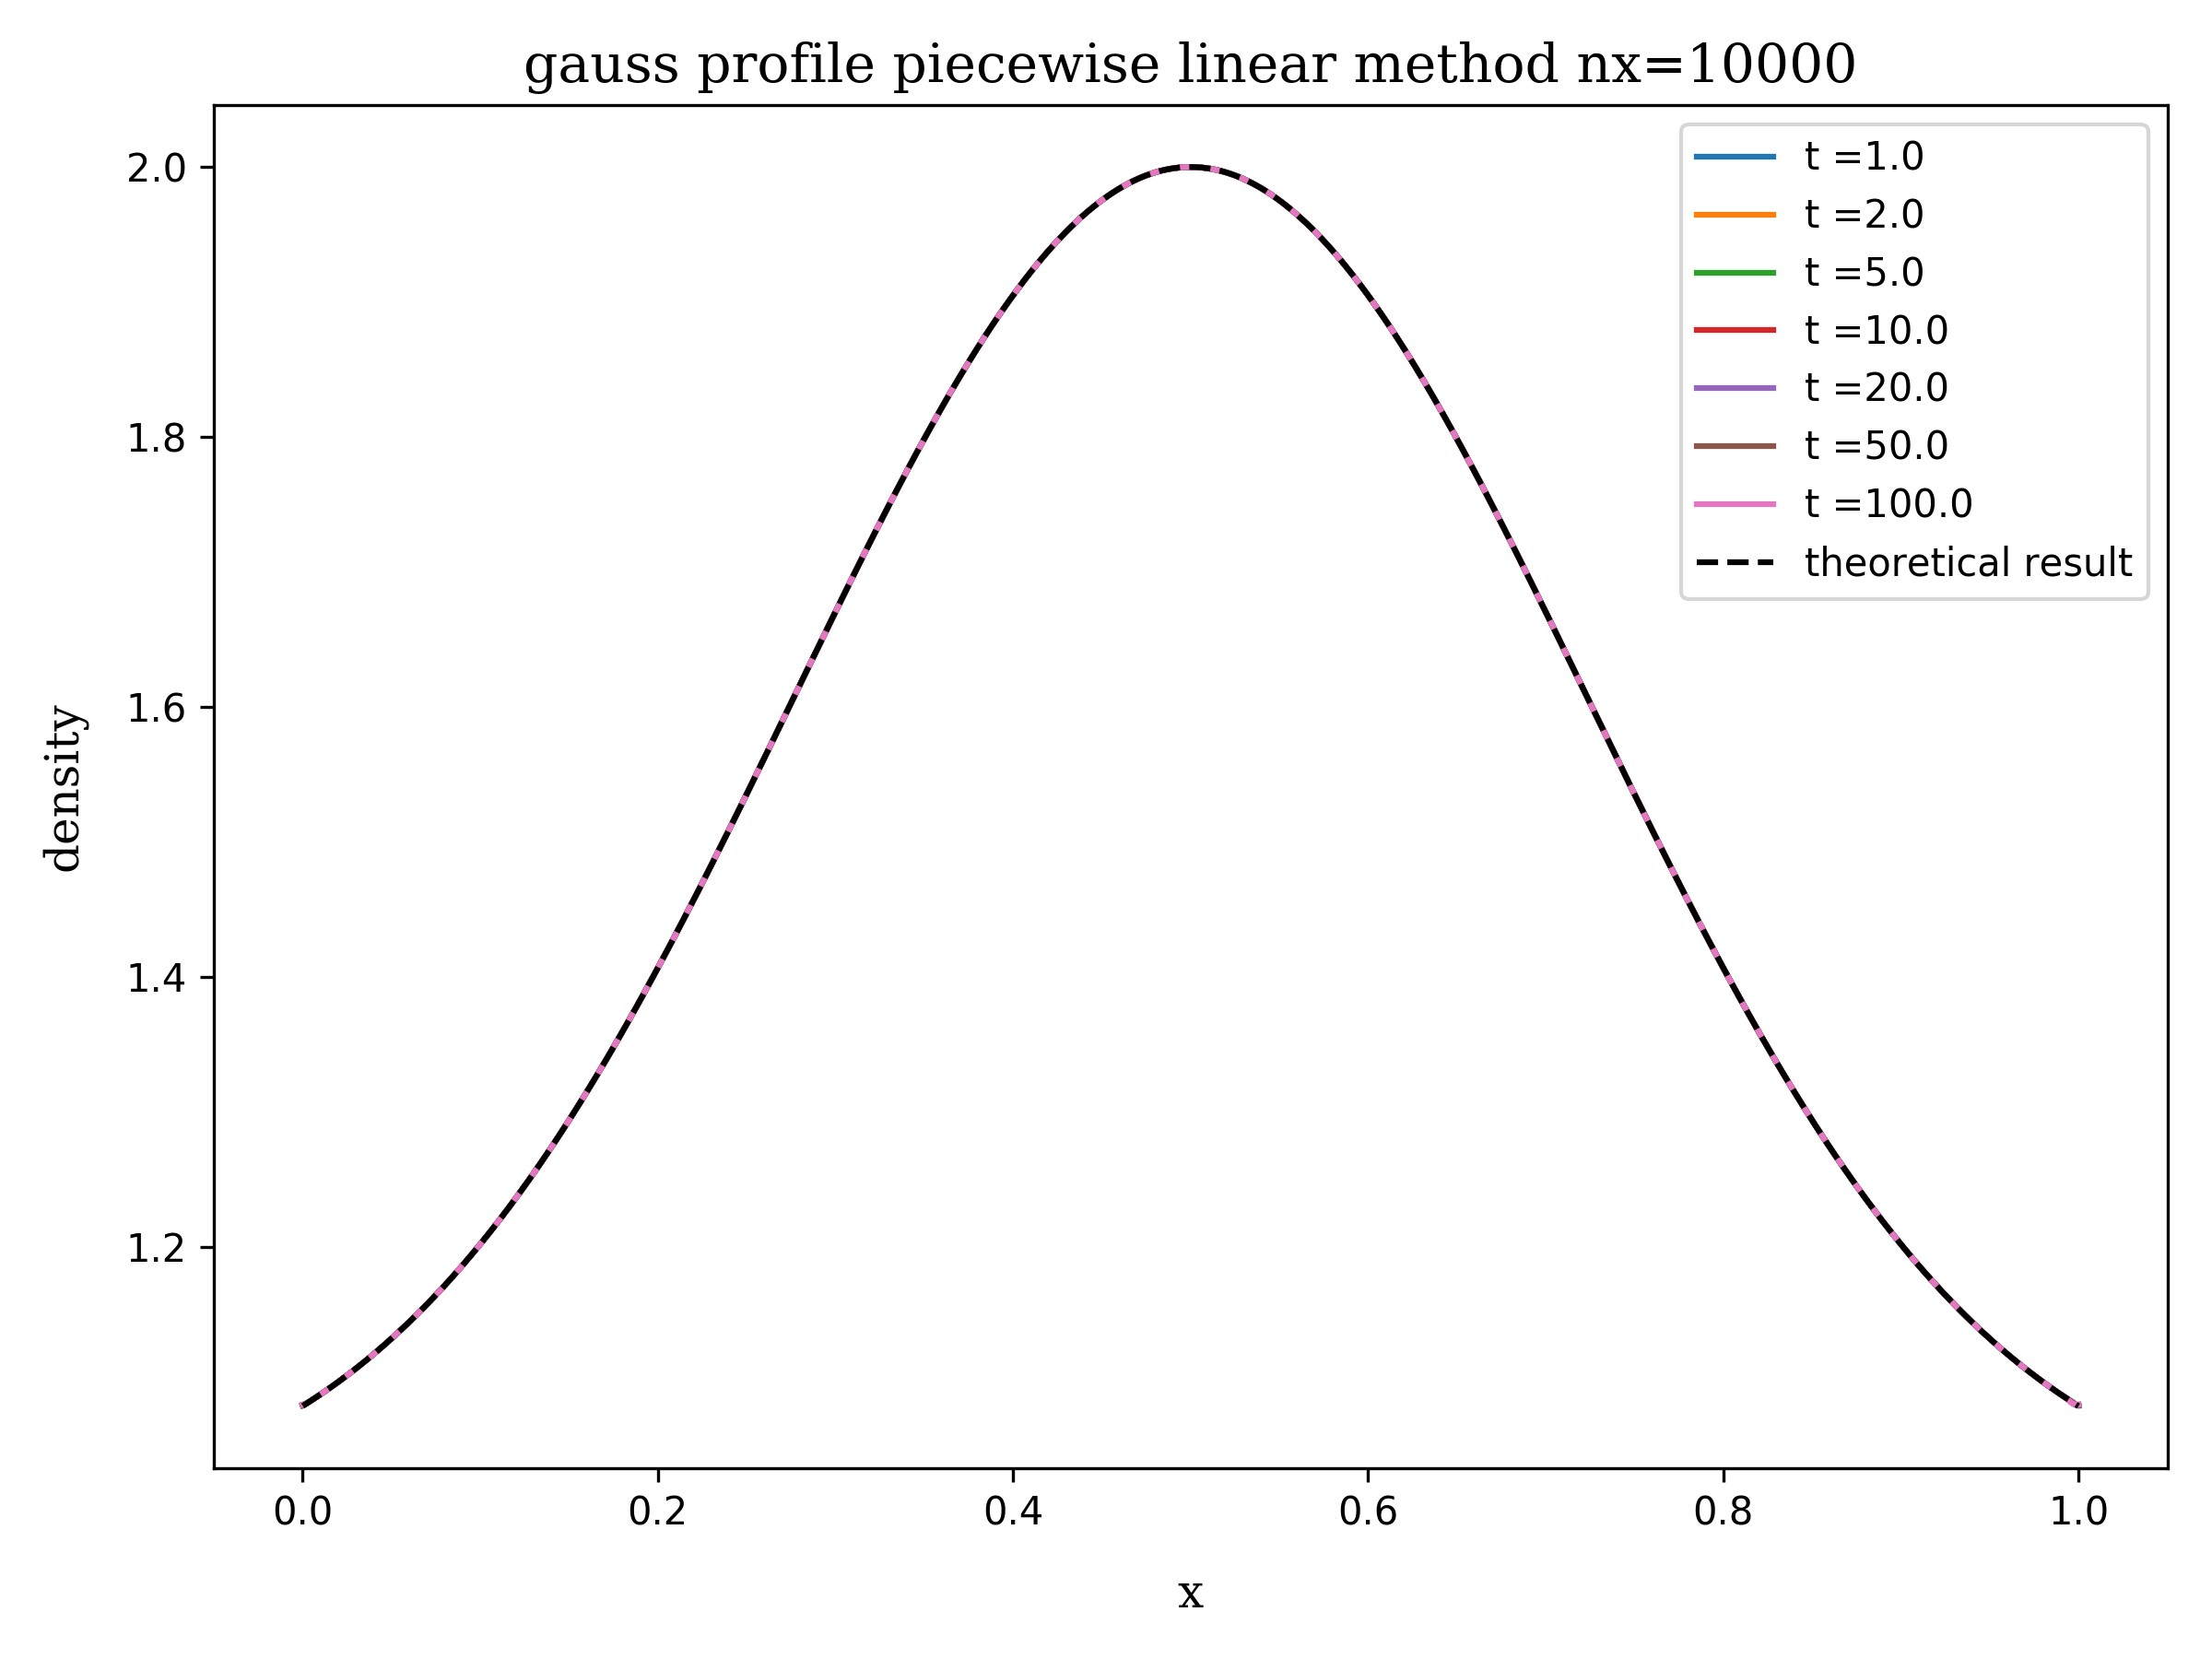
\includegraphics[height=.33\textheight]{../results/1D/pwlin/nx=10000/plot_advection_gauss_pwlin_nx=10000.png}
	\end{columns}
\end{frame}





\begin{frame}
	\begin{block}{New Problem: Oscillations}
		The piecewise linear elements can have overshoots, leading to the oscillations seen in the previous plots.

		
		\begin{center} 
			\includegraphics[height=0.2\textheight]{images/overshoot.png}
			
			\tiny{
				Image adapted from ``Lecture Numerical Fluid Dynamics'', Lecture given by C.P. Dullemond and H.H. Wang at Heidelberg University, 2009
			}
		\end{center}
			
		Godunov's theorem: \textit{any linear algorithm for
			solving partial differential equations, with the property of not producing new extrema, can be at
			most first order.}
		
		$\Rightarrow$ use non-linear conditions (slope limiters) to modify the slope $s_i^n$ to prevent overshoots. Requirement: total variation diminishing: $TV(\rho^{n+1}) \leq TV(\rho^n) \equiv \sum |\rho_i - \rho_{i-1}|$. Such a scheme will not develop oscillations near a jump, because a jump is a monotonically in/decreasing function and a TVD scheme will not increase the $TV$.
	\end{block}
\end{frame}